\section{Overview}
\begin{figure}[!ht]
\centering
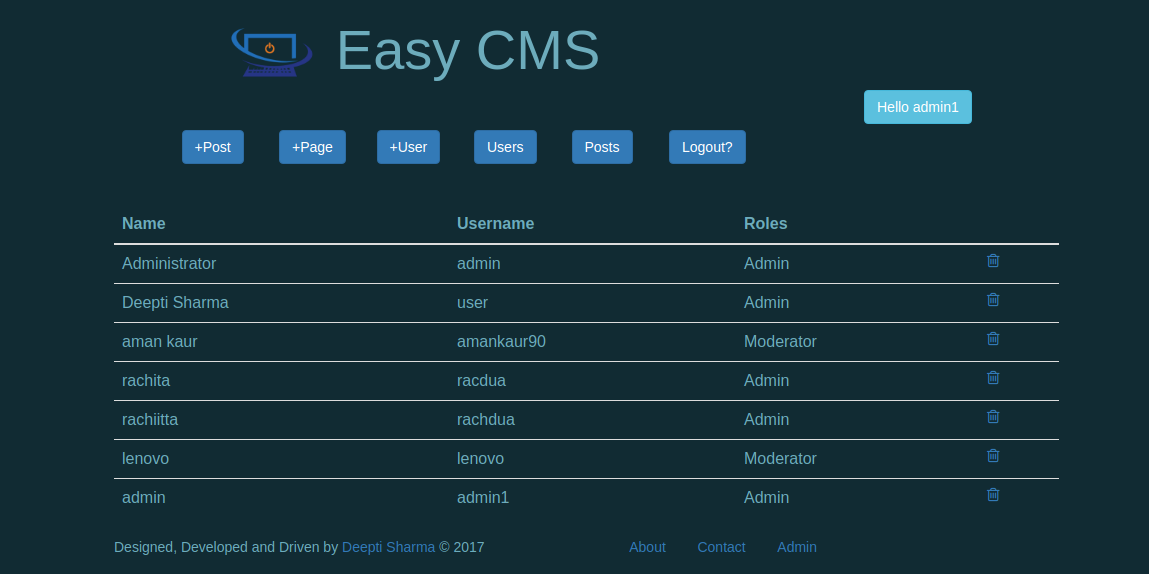
\includegraphics[scale=0.41]{input/images/new.png}                   
\caption{CMS}
\hspace{-1.5em}
\end{figure}
\subsection{What is CMS?}
The Content Management System (CMS) is a graphical user interface (GUI) that allows the user to control the creation, modification and removal of content from a website without needing to know anything about HTML.Here, CMS is an open-source interactive software application that supports the creation and modification of digital content. It is particularly designed for multiple users to use this system in a collaborative environment. \\\\
In addition, CMS can display data in different ways like entering text and listening sound. It
also has its own programming language which allows the system to be extended. It can
be thought of as a very powerful, programmable, graphical content storage system.\\
CMS makes it easy to put a wide range of data at a place which could help for future references allowing you to spend time experimenting and thinking about the wider problem.
Few famous CMS are: Wordpress, Drupal, Jumla etc. \\
The first ever CMS was RAINMAN (Remote Automated Information Network Manager) which was developed around in 1992. It was one of the first systems to allow content publishers to directly place their content into a live navigation hierarchy.
Dr. Glen Barry published the world's first blog in 1993 - "Forest Protection Blog" The term "weblog" was coined by Jorn Barger in Dec. 1997 Shortened to "blog" in 1999 by Peter Merholz.
\subsection{What CMS is not?}
CMS is designed to allow users to change most of the text, images, audio, & on your website without the need for a website developers assistance. Simple, everyday changes are now something you can do anytime, and anywhere you have an internet connection! Best of all, you don't need to to know HTML or any code to use a CMS.
This means that it can't ensure that your content is any good because it's job is just to manage the data. In terms of business, CMS can make executing your marketing plans easier and more efficient, but those plans still need to be conceived, created, and analyzed by a competent human. \\
This does not make the text better or worse, its just used for storing.
\subsection{Who uses CMS?}
Content Management Systems are widely used by engineers and scientists, in both industry and
academia for different purposes. Its even been used by business maintenance teams and various authors, for attracting the crowd and for promoting their work. There are way more reasons such as an income from blogs, common people's interest towards writing and much more.\\
 For example, Many well-known sites that are there who are powered by CMS:
\begin{itemize}
\item Forbes and ebay.
\item Sony and Microsoft news.
\item CNN hosts blogs for their many on-air personalities and for breaking news.
\end{itemize}
\subsection{Why CMS?}
The reason why I thought of creating a CMS of my own because I wanted to get a very specific idea of what it should do, and how it should work. Content Management System is a necessity nowadays for students as they have to write blogs for sake of daily diary as a part of their academic curriculum. Institutions can use this system to deploy on their server so that they can have a record of daily diaries of all the trainees and interns. It will develop a habit of writing in students. 

\section{The Existing System}
There are few existing systems which do the task like Wordpress or other softwares but
they don't have few features which I have added in this system. These system were not open source
and free web based software.
All exiting system suffers from at least one of the following system.
 \subsection{Limitations of previous system }
\begin{itemize}
\item No Speech Recognision Method. 

\item They are costly.

\item Don't provide direct pdf or other file saving options.

\item They need installation and a lot of system resources. 

\end{itemize}
\subsection{Advantages of making the system using PHP:}
\begin{itemize}
\item PHP was specially designed for a websites, the facilities that web designers typically want in a scripting language are built into it.
\item Another convenience is its handling of form input.
\item Accessing databases is just as easy. There are built-in facilities in PHP to access MySQL, Dbase, Oracle, InterBase, and so on.
\item When PHP scripts runs, If in case  you get error then messages will be like pinpointing the offending lines in your code to help you locate the error.
\end{itemize} 
\section{User Requirement Analysis}
\begin{enumerate}
\item Manage the content provided by user.
\item User can add text through both input and speech recognision method.
\item It can help many students, organisations, Institutions etc. to keep a track record of daily entries.
\item It provides a well secure method to add data.
\item It provides pdf document of the content added.
\end{enumerate}
\newpage


